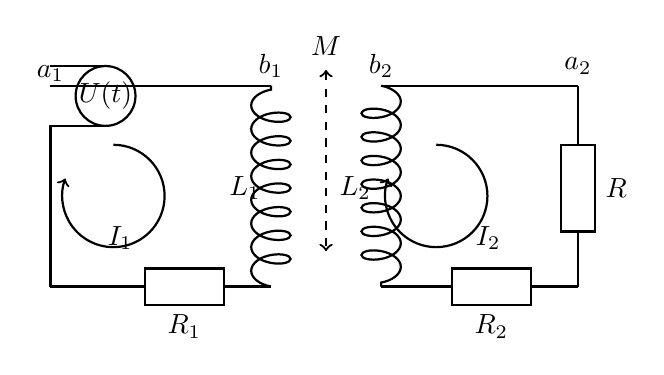
\begin{tikzpicture}[x=1cm,y=1cm,thick]
  % Coupled primary and secondary loops with distinct current arrows.
  \draw (0,0)--(0.7,0); \draw (0.7,-0.38) circle (0.38); \node at (0.7,-0.38) {$U(t)$}; \draw (0.7,-0.76)--(0,-0.76)--(0,-2.8);
  \draw (0,-2.8)--(1.2,-2.8); \draw[fill=white] (1.2,-3.03) rectangle (2.2,-2.57); \node[below] at (1.7,-3.03) {$R_1$}; \draw (2.2,-2.8)--(2.8,-2.8);
  \draw[decorate,decoration={coil,segment length=3mm,amplitude=2.5mm}] (2.8,-2.8)--(2.8,-0.25); \draw (2.8,-0.25)--(0,-0.25);
  \draw (4.2,-0.25)--(6.7,-0.25); \draw[decorate,decoration={coil,segment length=3mm,amplitude=2.5mm}] (4.2,-0.25)--(4.2,-2.8); \draw (4.2,-2.8)--(5.1,-2.8);
  \draw[fill=white] (5.1,-3.03) rectangle (6.1,-2.57); \node[below] at (5.6,-3.03) {$R_2$}; \draw (6.1,-2.8)--(6.7,-2.8);
  \draw (6.7,-2.8)--(6.7,-0.25); \draw (6.7,-1.0)--(6.7,-2.1); \draw[fill=white] (6.48,-2.1) rectangle (6.92,-1.0); \node[right] at (6.92,-1.55) {$R$};
  \node[left] at (2.8,-1.55) {$L_1$}; \node[left] at (4.2,-1.55) {$L_2$};
  \node at (3.5,0.25) {$M$}; \draw[<->,dashed] (3.5,-0.05)--(3.5,-2.35);
  \draw[->] (0.8,-1.0) arc[start angle=90,end angle=-200,radius=0.65] node[midway,left] {$I_1$};
  \draw[->] (4.9,-1.0) arc[start angle=90,end angle=-200,radius=0.65] node[midway,right] {$I_2$};
  \node at (0,-0.1) {$a_1$}; \node at (2.8,0) {$b_1$}; \node at (4.2,0) {$b_2$}; \node at (6.7,0) {$a_2$};
\end{tikzpicture}
